\section{Durchführung}
\label{sec:Durchführung}

\begin{figure}[ht]
    \centering
    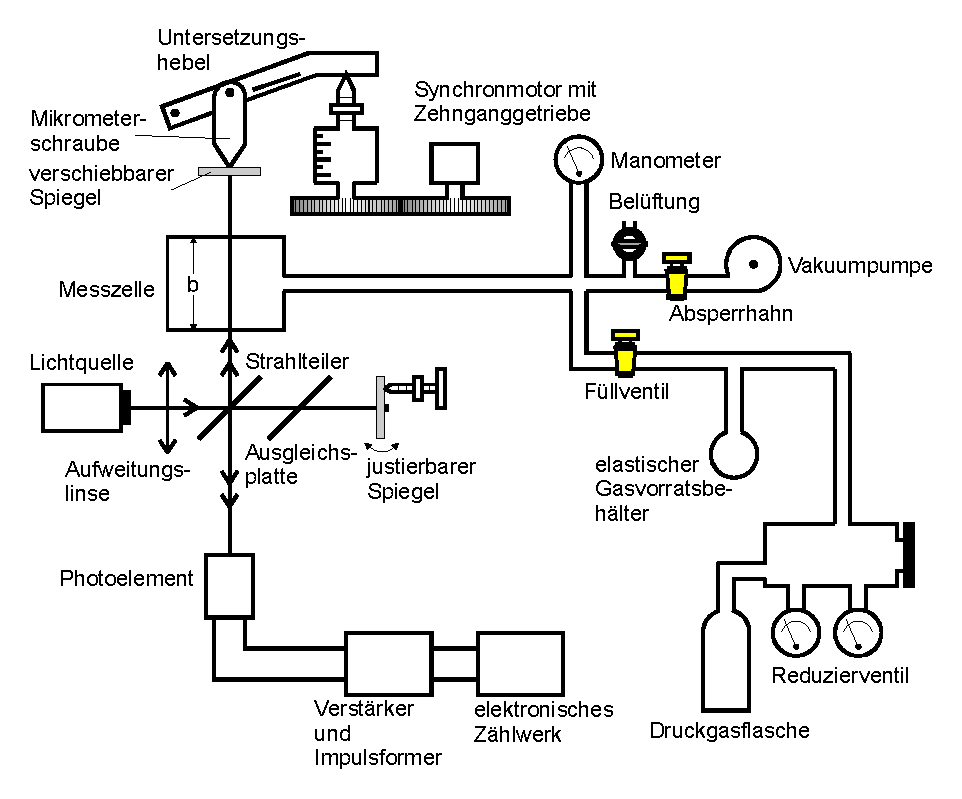
\includegraphics[width=0.9\linewidth]{pictures/Michelson3.pdf}
    \caption{Der grundlegende Aufbau eines Michelson Interferometers. \cite{v401}}
    \label{fig:Michelson3}
\end{figure}

Zunächst wird der in \autoref{fig:Michelson3} dargestellte Aufbau nachgebaut.
Dabei ist die Messzelle $b = 50 \unit{\milli\meter}$ lang und die Wellenlänge des Lasers beträgt $\lambda_\text{theo} = 635 \unit{\nano\meter}$.
Dann wird das Interferometer so justiert, dass die hellsten austretenden Strahlen an der Eintrittsstelle des Photoelements übereinander liegen.\\
Nun beginnt die eigentliche Messung.
Der Motor wird angeschaltet und läuft so lange, bis der Motor den Spiegel um 5 mm verschoben hat.
Die Impulse, die das Photoelement gemessen hat, werden notiert.
Dann wird der Motor wieder angeschaltet, jedoch mit umgekehrter Richtung.
Dadurch bewegt sich der Spiegel wieder die Strecke zurück.
Die Impulse werden wieder notiert.
Dieser Prozess wird 10 Mal wiederholt.

Bei er zweiten Messung wird der Spiegel an einer Stelle fixiert, der Motor ist also nicht mehr notwendig.
Nachdem die Zählung der Impulse auf Null gesetzt wurde, wird langsam durch eine Vakuumpumpe ein Vakuum in der Messzelle hergestellt.
Es wird bis $-600$ bar gepumpt.
Sind die $-600$ bar erreicht, wird der Zählerstand abgelesen.
Dann wird der Zählerstand wieder auf Null gestellt und die Messung wird nun in der umgekehrten Reihenfolge,
also von Vakuum zu Normaldruck, wiederholt.
Der Prozess wird in beide Richtungen 3 mal wiederholt.